\documentclass[12pt,letterpaper]{article}

% just for the example
\usepackage{lipsum}
% Set margins to 1.5in
\usepackage[margin=1.5in]{geometry}

% for graphics
\usepackage{graphicx}
\graphicspath{{./figures/}}

% for crimson text
\usepackage{crimson}
\usepackage[T1]{fontenc}

% setup parameter indentation
\setlength{\parindent}{0pt}
\setlength{\parskip}{6pt}

% for 1.15 spacing between text
\renewcommand{\baselinestretch}{1.15}

% For defining spacing between headers
\usepackage{titlesec}
% Level 1
\titleformat{\section}
  {\normalfont\fontsize{18}{0}\bfseries}{\thesection}{1em}{}
% Level 2
\titleformat{\subsection}
  {\normalfont\fontsize{14}{0}\bfseries}{\thesection}{1em}{}
% Level 3
\titleformat{\subsubsection}
  {\normalfont\fontsize{12}{0}\bfseries}{\thesection}{1em}{}
% Level 4
\titleformat{\paragraph}
  {\normalfont\fontsize{12}{0}\bfseries\itshape}{\theparagraph}{1em}{}
% Level 5
\titleformat{\subparagraph}
  {\normalfont\fontsize{12}{0}\itshape}{\theparagraph}{1em}{}
% Level 6
\makeatletter
\newcounter{subsubparagraph}[subparagraph]
\renewcommand\thesubsubparagraph{%
  \thesubparagraph.\@arabic\c@subsubparagraph}
\newcommand\subsubparagraph{%
  \@startsection{subsubparagraph}    % counter
    {6}                              % level
    {\parindent}                     % indent
    {12pt} % beforeskip
    {6pt}                           % afterskip
    {\normalfont\fontsize{12}{0}}}
\newcommand\l@subsubparagraph{\@dottedtocline{6}{10em}{5em}}
\newcommand{\subsubparagraphmark}[1]{}
\makeatother
\titlespacing*{\section}{0pt}{12pt}{6pt}
\titlespacing*{\subsection}{0pt}{12pt}{6pt}
\titlespacing*{\subsubsection}{0pt}{12pt}{6pt}
\titlespacing*{\paragraph}{0pt}{12pt}{6pt}
\titlespacing*{\subparagraph}{0pt}{12pt}{6pt}
\titlespacing*{\subsubparagraph}{0pt}{12pt}{6pt}

% Set caption to correct size and location
\usepackage[tableposition=top, figureposition=bottom, font=footnotesize, labelfont=bf]{caption}

% set page number location
\usepackage{fancyhdr}
\fancyhf{} % clear all header and footers
\renewcommand{\headrulewidth}{0pt} % remove the header rule
\rhead{\thepage}
\pagestyle{fancy}

% Overwrite Title
\makeatletter
\renewcommand{\maketitle}{\bgroup
   \begin{center}
   \textbf{{\fontsize{18pt}{20}\selectfont \@title}}\\
   \vspace{10pt}
   {\fontsize{12pt}{0}\selectfont \@author} 
   \end{center}
}
\makeatother

% Used for Tables and Figures
\usepackage{float}

% For using lists
\usepackage{enumitem}

% For using APA Citation format
\usepackage{apacite}

% Custom Quote
\newenvironment{myquote}[1]%
  {\list{}{\leftmargin=#1\rightmargin=#1}\item[]}%
  {\endlist}
  
% Create Abstract 
\renewenvironment{abstract}
{\vspace*{-.5in}\fontsize{12pt}{12}\begin{myquote}{.5in}
\noindent \par{\bfseries \abstractname.}}
{\medskip\noindent
\end{myquote}
}

\begin{document}

% Set Title, Author, and email
\title{Assignment P1}
\author{Snejana Shegheva \\ sshegheva3@gatech.edu}

\maketitle
\thispagestyle{fancy}

\begin{abstract}
In this assignment, we look at various interfaces and discuss them from the principles of human-computer interaction. We analyze Piazza's post filtering functionality from the perspective of a processor and predictor models. Then we contrast it with the participant view on the example of a podcast listening app. As we continue to explore the foundations of HCI principles, we move to the analysis of the feedback cycles by exploring Canvas's interfaces for submitting an assignment, and the effectiveness of its communication with the user to achieve their external goal. Designing good interfaces means aiming to reduce the gulfs of execution and evaluation through all their stages. We finally compare and contrast two activities with a large and small gulf of evaluations on the examples of Evernote and Google Photos apps. Immediate feedback on all user's activities can help bridge the gulf of evaluation by guiding their actions towards original intentions.  
\end{abstract}

\section*{Question 1 - Processor/Predictor User Models}
To explore the different type of user roles in interacting with interfaces, I selected Piazza's functionality for filtering posts based on the user's preference to prioritize the selection. Figure~\ref{fig::1} demonstrates the design that focuses on the user as a \textbf{processor} with the goal of making their post-reading more efficient. The outcome is faster access to the \textit{new} posts (if such filter is selected), that can be objectively measured, and evaluated with variations of filter functionality implementations. This feature, however, is directed towards a more experienced user who knows how to access the sub-menu. 

\begin{figure}[H]
\centering
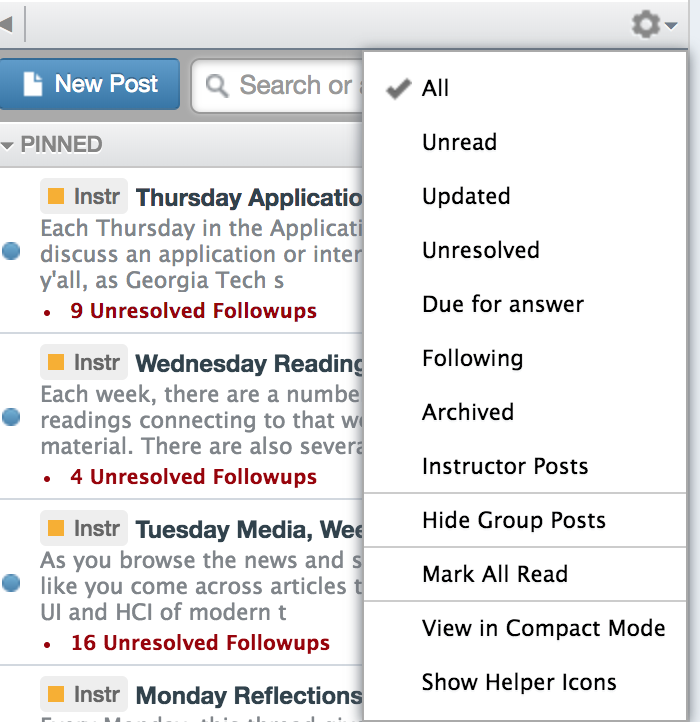
\includegraphics[width=2.5in, scale=.25]{piazza_filter.png}
\caption{Pizza's Post Filtering Functionality}
\label{fig::1}
\end{figure}

A closely related feature that treats the user as a \textbf{predictor} is shown in Figure~\ref{fig::2} that focuses on the user's perception. The user sees a blue dot next to some of the posts and predicts that those posts could be \textit{new}. The user can also interpret the icons on the right of the posts that signify a different type of post - question, note, or a poll. The predictor model allows the user to select posts to prioritize reading based on the \textit{popularity} (how many updates are in the post). User's expectations (such as the presence of student or instructor answer to the given question) upon clicking on the post are successfully met.  

\begin{figure}[H]
\centering
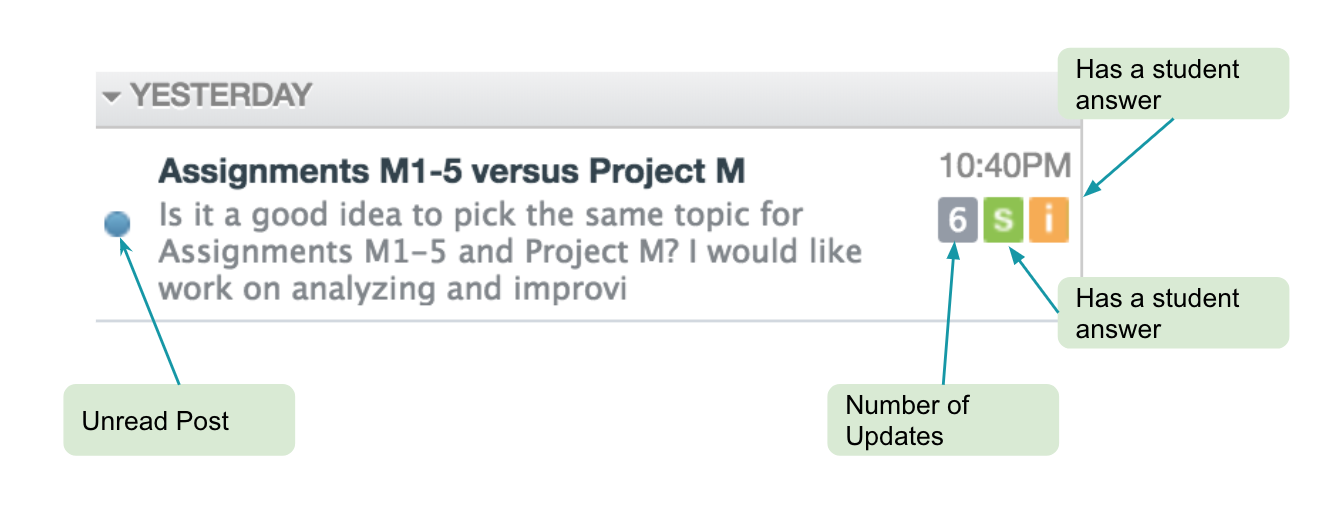
\includegraphics[width=4in, scale=.4]{piazza_predictor.png}
\caption{Pizza's Post Tagging Functionality}
\label{fig::2}
\end{figure}

Both perspectives of the interface allow user prioritizing which posts to read first. The predictor model is more suitable for a novice and provides a more qualitative approach for post selection. A further improvement to this model would be adding an indication that a post was authored by the user that would allow them to spot their own posts easier. Similarly, a filter for \textit{my posts} can be added for the processor model as well. As the user is reading the posts, it might be helpful to add a visualization that shows the ratio of read/unread posts on a daily basis so that the user can perceive the depth of their immersion in Piazza interactions.

\section*{Question 2 - Participant View}
Everyone listens to the podcasts. My favorite one is Joshua Weilerstein's podcast about classical music "Sticky Notes" \cite{sticky_notes}. I like listening to it on the Podcast Go App on my way to work that shifts a few different contexts of various durations - from the train ride that is relatively quiet to a noisy train station platform, from a peaceful park pathway to a busy street with loud car honking. Because the ambiance changes drastically, I need to either adjust volume in the transitions between the contexts, or pause the podcast altogether if the current context interferes with my hearing at the moment - for example, exiting the train while another train is departing from the same platform delivers enough noise that an image of commuters pressing palms against their ears is quite common.
Another example where the context changes more rapidly are announcements on the train about the upcoming stops. The message does not last more than a minute, but it could be that minute where Joshua Weilerstein said something critically important about the classical piece or composer being analyzed. And who could live with that?

The listening app has to be able to seamlessly fit into various contexts of my daily surroundings that may change rapidly (announcement, cars honking) or transitions more subtly (from a busy street into a quieter pathway). Depending on each situation I am in, the interface can be altered to perform with adjusted settings. 

Figure~\ref{fig::3} demonstrates three areas where the interface can be augmented to support transitioning into different contexts. A user should be to toggle between listening modes - quiet, normal, noisy - that automatically adjust volume for a better listening experience. This capability simplifies the volume control with a continuous nature to a discrete selection of the environment. When the context's changes are intermittent, toggling between modes might not be the most convenient feature. In such cases, the user can opt-in for seeing the audio transcript on the screen. This functionality reduces the chances of missing the critical content due to typical external interruptions. And, finally, the listener should be able to bookmark specific locations of the podcast to review them later at a more convenient time. The bookmarks can serve as both, pointers to the audio segment, and means to add comments. We do that with e-books already, but I have not come across this functionality in my podcast app. If you do, please kindly let me know. 

\begin{figure}[H]
\centering
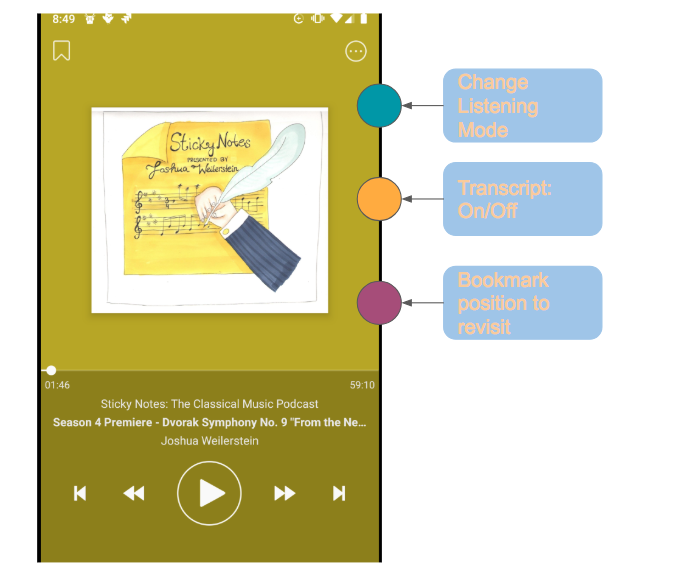
\includegraphics[width=4in, scale=.4]{podcast.png}
\caption{Podcast Listening App with three additional features: 1. Change Listening Mode (from quiet to noisy area). 2. Enable transcript mode when you expect sudden and brief interruptions. 3. Ability to bookmark audio position for later review.}
\label{fig::3}
\end{figure}



\section*{Question 3 - Feedback Cycles}

\subsection*{Gulf of Execution}
Don Norman identifies three stages in the Gulf of execution - plan, specify and perform \cite{norman2013design}. For the task of submitting an assignment to Canvas, we need to first map our external goal or intent (assignment submission) to a goal within the system. Canvas provides an excellent interface for identifying the intentions, suitable for even the novice user - locate the \textit{Assignments} menu -> select the upcoming Assignment -> Identify the big orange button \textit{Submit the Assignment}. This action is \textbf{easily discoverable}, even though it takes three steps to get to the point of uploading a file. Choosing a file from a local computer directory is consistent with other tools, and does not require training specific to Canvas only. It appears that Canvas provides additional means to bridge the gulf of execution for expert users - directly linking from your Cloud access, such as Google Drive or Dropbox. I can see that could be convenient if the user needs to submit multiple files and wishes to do so more efficiently than uploading files one by one\footnote{I have not tried the option of cloud linking, so I cannot attest to how well it works}. 

\subsection*{Gulf of Evaluation}
Gulf of evaluation includes its own three stages - perceive, interpret and compare \cite{norman2013design}. Within Canvas \textit{assignment submission} functionality there are two areas with a small and a vast gulf of evaluation. When a user attempts to submit an assignment \textit{without} selecting a file to upload, the system immediately gives feedback: "You must attach a least one file to this assignment" that is readily interpretable, and it matches user's expectation on the wrong action. This is an example of the small gulf of evaluation.

There is, however, secondary area, which hasn't satisfactorily bridged the gulf of evaluation. First, the user has no way of knowing if \textit{all} requirements for the assignment submission have been satisfied. Yes, the system indicated a successful upload of a file, but that is merely a subgoal. Are there more files the user should be submitting? Is the filename matching an expectation of the naming convention used for the assignment grading? The interface does not give a clear indication of the progress towards the final goal. Figure~\ref{fig::4} shows two sections that can be improved to communicate a better message to the user. In addition to "Due Date," the system can record and display a \textit{timestamp} of the submission that can indicate a successful submission. The page for the upcoming assignments changes by adding "Not Yet Graded" message. The user perceives this as a state change, but does necessarily interpret it as "assignment submitted." There is not enough information to compare what was wanted "submit the assignment" with what has happened. This gulf of evaluation can be bridged by sending a confirmation email of the completed submission.

\begin{figure}[H]
\centering
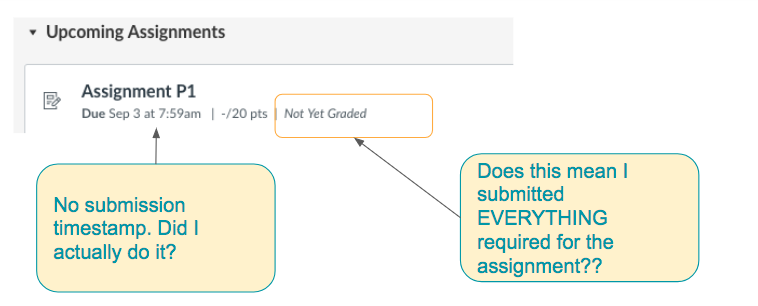
\includegraphics[width=4in, scale=.4]{canvas.png}
\caption{Canvas assignments page}
\label{fig::4}
\end{figure}

\section*{Question 4 - Narrowing the Gulf of Evaluation}
One of my favorite apps, Evernote \cite{evernote} that has an overall straightforward and intuitive interface struggles with a vast gulf of evaluation in one particular area of note editing. The user can edit notes across devices, expecting the app to take care of seamless synchronization. ISSUE - When a user updates the same note on two different devices (not even simultaneously), and the sync did not execute successfully, and user is left with feedback like the one seen in Figure~\ref{fig::5}. 

\begin{figure}[H]
\centering
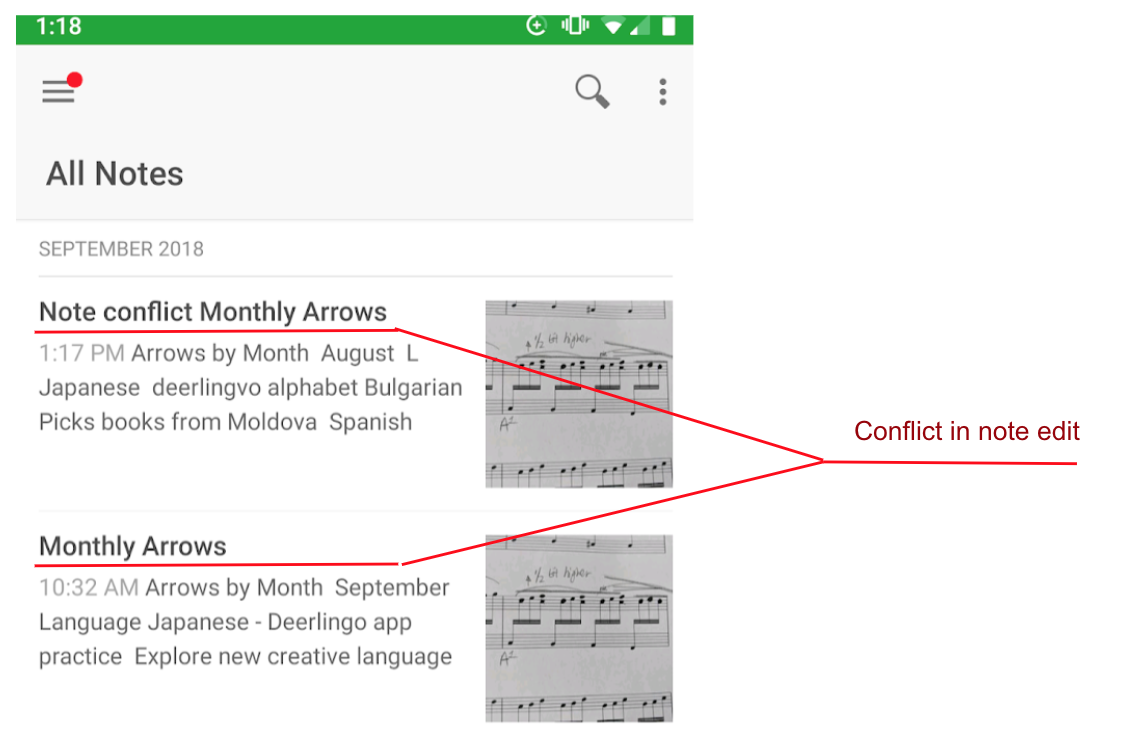
\includegraphics[width=4in, scale=.4]{evernote.png}
\caption{Evernote Conflict}
\label{fig::5}
\end{figure}

The user perceives the state but receives no guidance on correcting the observed issue. Trying the make sense of what happened, i.e., find the offending lines, is not possible where the two notes are presented separately without a comparative view. The user had an explicit goal of execution - make a few edits to the note, but upon failure, did not know how to make corrective actions.

\begin{figure}[H]
\centering
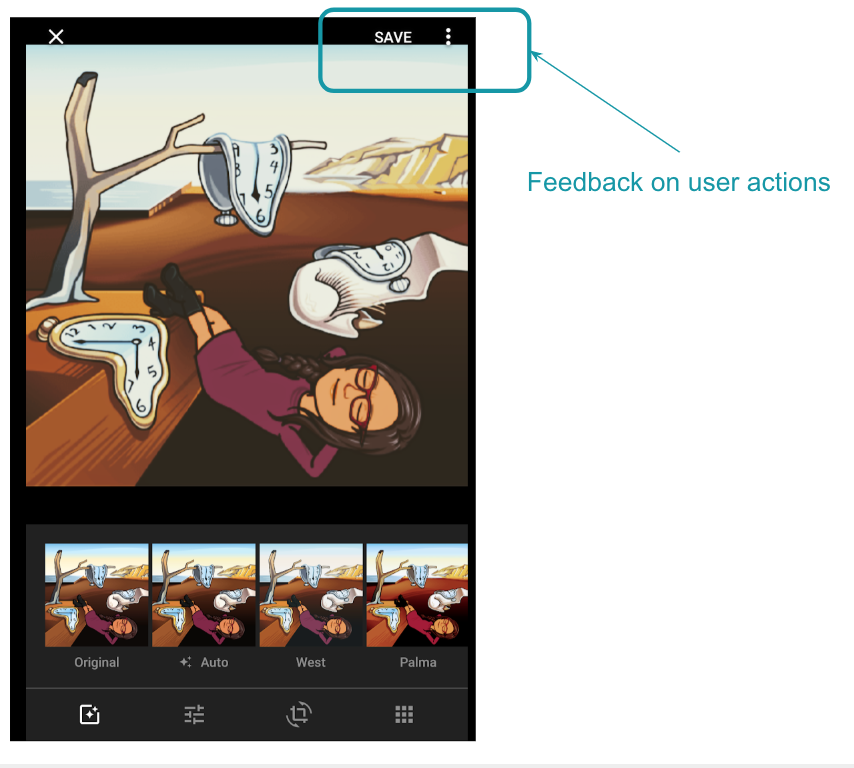
\includegraphics[width=3in, scale=.3]{photo.png}
\caption{Image Edits with Google Photo's App}
\label{fig::6}
\end{figure}

Let's compare the Gulf of evaluation for the Evernote app to that of Google Photo's app \cite{photos}. When the user edits a photo, immediate feedback on the action is given by showing \textit{SAVE} button (previously invisible) that suggests that user had introduced changes that haven't been saved yet. Interpreting the state, and comparing the results with the user's intentions bridges the gulf of evaluation, and makes a good user experience. 

What could Evernote do better? Conflict resolution in itself could be a significant feature with multiple steps to guide the successful resolution. A one step before that is adding feedback upon edit for whether or not the note has been synced. Seeing this on the device where the note is edited would give the user an indication on the note's current state. Subsequently, when the user switches to a different device, the interface can provide feedback, other than just a timestamp of the last sync, that user can use compare to their expectations. For example, introduce a status for a note that tracks its recency and/or source of a recent update. For advanced users, the evaluation gulf may be reached by providing access to user activity logs for the user to trace their changes and resolve the conflicts manually if necessary. 

\bibliographystyle{apacite} 
\bibliography{bibtemp}

\end{document}
